\documentclass{article}
\usepackage{amsmath, amsthm, amssymb}
\usepackage{bibentry}

% \usepackage{../code/algorithmicx/algpseudocode}
% \usepackage{algpseudocodex}
\usepackage{algorithmic}
\usepackage{algorithm}

\usepackage{tikz, xcolor}
\usetikzlibrary{lindenmayersystems}

\newcommand{\del}{\partial}
\newcommand{\eps}{\varepsilon}
\newcommand{\disk}{\mathbb{D}}
\newcommand{\reals}{\mathbb{R}}
\newcommand{\cnums}{\mathbb{C}}
\newcommand{\red}[1]{\textcolor{red}{#1}}
\newcommand{\green}[1]{\textcolor{green}{#1}}

\newtheoremstyle{custom}{3mm}{3mm}{\normalfont}{0pt}{\bfseries}{}{\newline}{}
\theoremstyle{custom}

%\newcommand{\mydef}[1]{\indent\textbf{Definition.}\newline #1\par}
\newtheorem{definition}{Definition}
\newtheorem{theorem}{Theorem}[section]
\newtheorem{lemma}[theorem]{Lemma}
\newtheorem{corollary}[theorem]{Corollary}
\newtheorem{proposition}[theorem]{Proposition}
\newtheorem{remark}{Remark}
\begin{document}

\begin{titlepage}
    \centering
    \Huge \textbf{Conformal Mesh Mappings}\\
    \vspace{15cm}
    \Large Bachelor Thesis D-MATH ETHZ \\
    \Large Alessandra Iacopino \\

    \Large Supervisor: Prof. Dr. Ralf Hiptmair \\
\end{titlepage}

\begin{abstract}
    When performing shape optimization one encounters the problem of conformal mapping of a relatively simple onto a potentially very complicated domain. The Riemann mapping theorem guarantees the existence of such a conformal map, but does not provide any explicit construction of it. In practice, one has to resort to numerical methods to construct the conformal map.
    This text is intended to give a general overview of currently known numerical algorithms for this very problem, and to provide a comparison of their suitability in terms of input and output format as well as their performance in terms of accuracy and speed.
    One of the algorithms is then implemented in the context of a 2-dimensional shape optimization problem, and its performance is evaluated.


    % If the region S is a convex polygon, the extremal problem can be treated numerically by linear programming methods (Opfer [202]).
\vspace{3cm}

    Keywords: 
    numerical conformal mapping, 
    Riemann mapping theorem, 
    Schwarz-Christoffel mapping, 
    conjugate function method, 
    Fourier series representation, 
    curvilinear triangular mesh, 
    mesh generation, 
    finite element method, 
    Laplace-Beltrami equations, 
    spectral conformal parameterization, 
    Ricci flow, 
    charge simulation method, 
    RT-algorithm, 
    CRDT(cross-ratios Delaunay triangulation)
    https://observablehq.com/@jrus/scpie
    
\end{abstract}
\newpage

\tableofcontents
\newpage

% \section{Introduction}
\subsection{Motivation}
why i care, target audience
\subsection{Problem Setting}
\section{Theoretical Background}
%maybe change structure to section existence of a conformal map, section construction of a conformal map

\subsection{Conformal Mappings}

\begin{definition}
    A \textbf{conformal mapping}, also called a conformal map, conformal transformation, angle-preserving transformation, or biholomorphic map, is a transformation $f(z)$ that preserves local angles. An analytic function is conformal at any point where it has a nonzero derivative.
\end{definition}

This type of mapping is useful as some mesh properties remain regular under such transformations. This ensures that cells do not become too stretched or overlap, which would cause numerical issues or even solver failure \cite{Wechsung2019}. 
In two dimensions, conformality can be achieved by enforcing that the mapping satisfies the Cauchy-Riemann equations. 

\begin{definition}
    We call a subset $\Omega \in \mathbb{C}$ \textbf{proper} if $\emptyset \neq \Omega \neq \mathbb{C}$.
\end{definition}

\begin{theorem}[\cite{Wegmann2005}, p. 357] \label{thm:ExtensionToBoundary}
    The conformal mapping $\Phi:D\to G$ can be extended to a continuous mapping $\Phi:\bar{D}\to\bar{G}$ if and only if the boundary $\Gamma$ of $G$ consists of a closed curve.
\end{theorem}


\subsection{Riemann Mapping Theorem}
The reason why we use conformal mappings for shape optimisation in two dimensions is the following
\begin{theorem}[Riemann Mapping Theorem]
    If $\Omega$ is a non-empty simply connected open proper subset of the complex plane $\mathbb{C}$, then there exists a biholomorphic mapping $f$ (i.e. a bijective holomorphic mapping whose inverse is also holomorphic) from $\Omega$ onto the open unit disk
    $$ D = \{z \in \mathbb{C}: |z|<1 \}. $$
    This mapping is known as a Riemann mapping.
\end{theorem}

The beauty of the Riemann mapping theorem lies in its weight of implications, i.e. the fact that it guarantees the existence of a conformal map between any two simply connected domains in the complex plane, provided they are not the entire plane. The existence of this Riemann map is a priori not obvious: Even relatively simple Riemann mappings (for example a map from the interior of a circle to the interior of a square) have no explicit formula using only elementary functions.
Simply connected open sets in the plane can be highly complicated, for instance, the boundary can be a nowhere-differentiable fractal curve of infinite length, even if the set itself is bounded. One such example is the Koch curve. The fact that such a set can be mapped in an angle-preserving manner from the nice and regular unit disc seems counter-intuitive.
\bigskip
\begin{center}
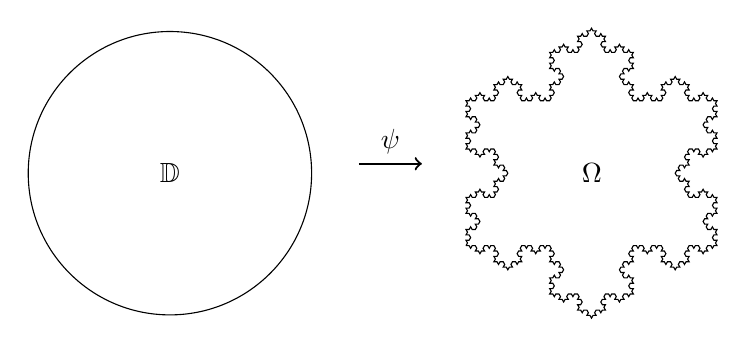
\begin{tikzpicture}[scale=0.8]
    \pgfdeclarelindenmayersystem{Koch curve}{
        \rule{F -> F-F++F-F}
        }
        \draw [black, xshift=6.7cm]
    [l-system={Koch curve, step=1.4pt, angle=60, axiom=F++F++F, order=4}]
    lindenmayer system -- cycle;

    \pgfmathsetmacro{\kochwidth}{2pt*4*8}
    \draw [black] (2,1.15) circle (\kochwidth pt);
    \node at (2,1.15) {$\disk$};
    \node at (8.7,1.15) {$\Omega$};

    \draw [->, thick] (5,1.3) -- (6,1.3) node [midway, above] {$\psi$};
\end{tikzpicture}
\end{center}
\bigskip

The existence of a conformal map between any two simply connected, open proper subsets of $\mathbb{C}$ is what allows us to perform shape optimisation in two dimensions by solving the optimisation problem on a simple reference domain (e.g. the unit disk) and then mapping the solution to the complicated target domain.
We closely follow the proof by normal families in \cite{SteinShakarchi2003}.
\subsubsection{Preliminary Results}
\begin{lemma}[Schwarz Lemma] \label{thm:SchwarzLemma}
    Let $f:\disk\to\disk$ be holomorphic with $f(0) = 0$. Then 
    \begin{enumerate}
    \item $|f(z)| \leq |z|$ for all $z \in \disk$.
    \item If for some $z_0\neq 0$ we have $f(z_0)=z_0$ then f is a rotation.
    \item $|f'(0)| \leq 1$ and if equality holds, then $f$ is a rotation.
    \end{enumerate} 
\end{lemma}
\red{\textit{Proof.?}}

\begin{definition}
    A family $\mathcal{F}$ of holomorphic functions on a domain $\Omega$ is called \textbf{normal} if every sequence in $\mathcal{F}$ contains a subsequence that converges uniformly on any compact subset of $\Omega$.
\end{definition}    
\begin{definition}
    A family $\mathcal{F}$ is called \textbf{uniformly bounded on compact subsets} of $\Omega$ if for every compact subset $K \subset \Omega$ there exists a constant $M_K$ such that $|f(z)| \leq M_K$ for all $z \in K$ and all $f \in \mathcal{F}$.
\end{definition}
\begin{definition}
    A family $\mathcal{F}$ of holomorphic functions on a domain $\Omega$ is called \textbf{equicontinuous} if for every $\epsilon > 0$ there exists a $\delta > 0$ such that if $z \in \Omega$ with $|z-z_0| < \delta$ we have $|f(z) - f(z_0)| < \epsilon$ for all $f \in \mathcal{F}$.
\end{definition}
\begin{theorem}[Montel]
    A family $\mathcal{F}$ of holomorphic functions on $\Omega$ that is uniformly bounded on compact subsets of $\Omega$ is normal if and only if it is equicontinuous on compacta.
\end{theorem}
\red{\textit{Proof.?}}

\begin{proposition}[Uniform Convergence to Holomorphic Limit and Injectivity]
    Let $\Omega \subset \mathbb{C}$ be a connected open subset and let $f_n: \Omega \to \mathbb{C}$ be a sequence of injective holomorphic functions that converges uniformly on compact subsets of $\Omega$ to a holomorphic function $f$. Then $f$ is either constant or injective.
\end{proposition}

\begin{proposition}[Cauchy Inequality]
\label{thm:CauchyInequality}
    Let $f$ be holomorphic on an open set containing the closure of a ball $B_R(z_0)$ centered at $z_0$ of radius R. Then $$ |f^{(n)}(z_0)|\leq \frac{n! \lVert f \rVert _C}{R^n},$$ where $ \lVert f \rVert _C= \displaystyle \sup_{z\in C}|f(z)|$ on the boundary circle $C$.
\end{proposition}

\red{\textit{Proof.?}}

\begin{theorem}[Implicit Mapping Theorem \cite{EinsiedlerWieser2022AnalysisSkript}, p.573] \label{thm:ImplicitMappingTheorem}
    Let $r > 0$ be a radius, and let $x_0 \in \mathbb{R}^n$, $y_0 \in \mathbb{R}^m$. Consider the open set $W = B_r(x_0) \times B_r(y_0) \subset \mathbb{R}^n \times \mathbb{R}^m$ defined as
$$
W = \{ (x, y) \in \mathbb{R}^n \times \mathbb{R}^m : \| x - x_0 \|_2 < r \text{ and } \| y - y_0 \|_2 < r \}.
$$
Let $F: W \to \mathbb{R}^m$ be a continuous function satisfying the following conditions:
\begin{enumerate}
    \item $F(x_0, y_0) = 0$.
    \item The partial derivatives $\partial_{y_k} F : W \to \mathbb{R}^m$ exist for all $k \in \{1, \dots, m\}$ and are continuous on $W$.
    \item The partial differential $D_y F(x_0, y_0)$ (the differential of the map $y \mapsto F(x_0, y)$ at $y_0$) is invertible.
\end{enumerate}
Then there exist radii $\alpha, \beta \in (0, r)$ such that for the open balls $U_0 = B_\alpha(x_0) \subset \mathbb{R}^n$ and $V_0 = B_\beta(y_0) \subset \mathbb{R}^m$, there exists a unique continuous function $f: U_0 \to V_0$ satisfying:
\begin{itemize}
    \item $f(x_0) = y_0$.
    \item For all $(x, y) \in U_0 \times V_0$, we have 
    $$ F(x, y) = 0 \quad \text{if and only if} \quad y = f(x). $$
\end{itemize}
\end{theorem}


\subsubsection{Proof of Riemann Mapping Theorem}
\textit{Step 1: Existence of a bounded injective conformal map to the unit disk} \\
Let $\Omega$ be a simply connected open proper subset of $\mathbb{C}$. We show that $\Omega$ is conformally equivalent to an open subset of the unit disk containing the origin. 
Indeed, choose $\alpha \notin \Omega$ and consider the function $f(z) = log(z-\alpha)$ on $\Omega$, which is well-posed and holomorphic since $z-\alpha$ never vanishes on $\Omega$. 
Note $f$ is injective since $e^{f(z)} = z-\alpha$ ($f(z_1) = f(z_2) \implies z_1 - \alpha = z_2 - \alpha$).
Then for a point $\omega \in \Omega$ we get $f(z) \neq f(\omega) + 2\pi i \forall z \in \Omega$ since otherwise we would find $z = \omega$ again by exponentiating.
In fact, $f(z)\cap B_{\epsilon}(f(\omega) + 2\pi i) = \emptyset$ for some $\epsilon > 0$ since otherwise we would find a sequence $z_n \to \omega$ with $f(z_n) \to f(\omega) + 2\pi i$, contradicting the continuity of $f$.
Finally, the function $g(z) = \frac{1}{f(z) - (f(\omega) + 2\pi i)}$ is well-defined, holomorphic and injective on $\Omega$ and maps $\Omega$ to a bounded subset $g(\Omega)\subset\mathbb{C}$, so $g$ is conformal. By boundedness of $g(z) < \frac{1}{\epsilon}$ we can scale and translate $g(\Omega)$ to contain the origin and fit into the unit disk.

\textit{Step 2:} \\
By step 1 we can assume $\Omega$ to be an open subset of the unit disk with $0\in\Omega$.
Consider the family $\mathcal{F}$ of all injective holomorphic functions $f: \Omega \to \mathbb{D}$ with $f(0) = 0$.
Note that $\mathcal{F}\neq\emptyset$ since it contains the identity, and it is a uniformly bounded family by construction (maps into unit disk). 
We now want to find a function $f \in \mathcal{F}$ that maximizes $|f'(0)|$. \red{(WHY?)}
Observe that by the Cauchy inequality \red{ \ref{thm:CauchyInequality}} $|f'(0)|$ are uniformly bounded for $f$ in $\mathcal{F}$.
\red{Next, let $$s:= \displaystyle \sup_{f\in\mathcal{F}} |f'(0)|.$$ and choose a sequence {$f_n$}$\subset\mathcal{F}$ such that $|f_n'(0)| \to s$ as $n\to\infty$.}
By Montel's theorem, {$f_n$} has a subsequence converging uniformly on compacta to a holomorphic $f$ on $\Omega$.
Since $s\geq 1$ (the identity is in $\mathcal{F}$), $f$ is non-constant and by the proposition on uniform convergence to holomorphic limit and injectivity, $f$ is injective.
By continuity we have $|f(z)\leq 1$ for all $z\in\Omega$, and by the \red{maximum modulus principle} $|f(z)|<1$.
Finally and since $f(0) = 0$, we have $f\in\mathcal{F}$ and $|f'(0)| = s$.

\textit{Step 3: $f$ is a conformal map from $\Omega$ to $\mathbb{D}$.} \\
By step 1 we have injectivity, hence it suffices to show $f$ is surjective.
Suppose towards a contradiction that $f$ is not surjective, we will construct a function in $\mathcal{F}$ with derivative greater than $s$ at the origin.
So let $\alpha\in\mathbb{D}$ be such that $\alpha\notin f(\Omega)$ and consider the automorphism of the unit disk that interchanges 0 and $\alpha$,
$$\psi_{\alpha}(z) = \frac{\alpha-z}{1-\bar{\alpha}z}.$$
Since $\Omega$ is simply connected and by continuity of $f$ and $\psi_{\alpha}(\Omega)$, the set $U:= (\psi_{\alpha}\circ f)(\Omega)$ is simply connected and does not contain the origin.
Thus we can define a square root function on $U$ by $$ q(w)=e^{\frac{1}{2}log w}.$$
Next, consider the function $$F=\psi_{q(\alpha)}\circ q \circ \psi_{\alpha}\circ f.$$
Then $F\in\mathcal{F}$ since $F(0) = 0$ and $F$ is holomorphic and injective since all the composing functions are. Also, $F$ maps into the unit disk since all the composing functions do.
But now if $h$ denotes the square function $h(w)=w^2$, then we must have $$f = \psi_{\alpha}^{-1}\circ h \circ \psi_{q(\alpha)}^{-1} \circ F = \Psi \circ F.$$
But $\Psi:\mathbb{D}\to\mathbb{D}$ satisfies $\Psi(0) = 0$ and is not injective since $F$ is but $h$ is not. 
By the Schwarz lemma \ref{thm:SchwarzLemma} we get $|\Psi'(0)| < 1$ and hence
$$|f'(0)| = |\Psi'(0)||F'(0)| < |F'(0)|,$$
contradicting maximality of $|f'(0)|$ in $\mathcal{F}$.

Finally, multiplying $f$ with a suitable unimodular complex number gives the desired conformal map from $\Omega$ to $\mathbb{D}$ with $f(0) = 0$ and $f'(0) > 0$. $\hfill\qed$

\begin{corollary}
    Any two simple connected open proper subsets of $\mathbb{C}$ are conformally equivalent.
\end{corollary}
\textit{Proof.} This follows directly from the Riemann mapping theorem by taking the unit disk as an intermediate step.
$\hfill\qed$ \\
 \\
This completes the theory for why shape optimisation of two dimensional simply connected regions works in the first place.
Here follows some more theory on how to actually construct such conformal maps numerically.

Existence established, the problem now becomes the explicit construction of a conformal mapping. A priori there are infinitely many conformal mappings from $\mathbb{D}$ to any simply connected bounded region $\Omega$, which is why the introduction of boundary conditions is needed to get uniqueness of $\Phi$ and thus well-posedness of the problem. This results in the problem being translated into solving a Boundary Value Problem (BVP) for analytic functions. 


% \red{add section 2.5:} error of operator K_N for methods based on function conjugation
\subsection{Boundary Value Problems}\label{chap:BoundaryValueProblems}\label{operatorK_N}
In Riemann's thesis, conformal mappings are a mere special case of the more general family of boundary value problems of analytic functions on the unit disk $D$ or in its exterior $D^{-}:=\{z: |z|>1\}$. The simplest such problem can be described as finding $\Psi$ analytic in $D$, continuous in $\bar{D}$ and satisfying $$Re(\Psi(e^{it}))=\psi(t)$$ on the boundary of $D$, where $\psi$ is $2\pi$-periodic and Hölder continuous
This problem has a unique solution up to an imaginary constant, which can be constructed using the conjugation operator $$K\Psi(s) := \frac{1}{2\pi}\int_{0}^{2\pi} \Psi(t)cot(\frac{s-t}{2}) dt,$$ which is also known as \red{Hilbert Transform}.
In order to use numerical methods efficiently via the \red{Fast Fourier Transform def?} we will prefer the functions' Fourier series representations. Hence on a grid of $N = 2n$ equidistant \red{why? FFT requires it? has crowding as an effect...} points $t_j = \frac{(j-1)2\pi}{N}$, $\Psi$ will be written as $$\Psi(t_j)=\sum_{k=-n+1}^{n} c_k e^{ikt_j} \text{ for } j\in [N]$$ and the conjugation operator can be approximated by the operator $K_N$ defined as $$K_N\Psi(t_j) = \sum_{k=1}^{n-1} -i c_k e^{ikt_j} + ic_{-k} e^{-ilt_j}.$$
The function $K_N$ is thus defined as a trigonometric polynomial obtained by interpolating $\Psi$ at the grid points. This approximation of the actual operator $K$ satisfies $$\|K \Psi - K_N \Psi\|_{\infty} \in O(n^{-\alpha+1/2}) $$ for $\Psi\in C^{\alpha}$ Hölder continuous.
If $\Psi$ is smoother, e.g. $\Psi \in C^{k-1}$, the error decreases to $$\|K \Psi - K_N \Psi\|_{\infty} \in O(n^{-k}log(n) \|\Psi^{(k)}\|_{infty})$$ \cite{Wegmann2005} p. 362.
\red{add more details on this operator?}

\subsection{Hilbert Transform \cite{Castillo2025}}
\red{probably way too much detail}
\subsection{Mixed boundary conditions (Wec 4.3)(?)}
\subsection{Hilbert theory and different inner products}

From complex analysis we know that a complex differentiable function with nonvanishing complex derivative is conformal, and complex differentiability in two dimensions can be caracterised by the Cauchy-Riemann equations (necessary and sufficient condition).
Denoting 
$$B:= \begin{pmatrix}
    \partial_x & -\partial_y \\
    \partial_y & \partial_x
\end{pmatrix}$$
we want to find a deformation $\Phi$ such that $B\Phi = 0$.

As a byproduct of the Cauchy-Riemann equations, both components of a conformal map are harmonic functions, i.e. they satisfy Laplace's equation $\Delta u = 0$.
Thus, one way to construct conformal maps is to solve Laplace's equation with suitable boundary conditions. \ref{chap:BoundaryValueProblems}

The Cauchy-Riemann equations however do not guarantee a solution for arbitrary boundary data. A holomorphic map from the boundary of the unit disk onto some boundary of a convex set in $\mathbb{R}^ 2$ satisfies Cauchy-Riemann equations if the boundary of the target set can be described by non-negative Fourier frequencies [PROOF]. Thus, the choice of parametrization of the target region's boundary is another challenge posed when solving conformal mapping problems, along with finding a holomorphic deformation $\Phi$.

In order to keep the approximation error as low as possible while maintaining good solver performance, we typically want uniform meshes, e.g. where the triangulation is close to equilateral. The quality of a mesh is measured in terms of its individual cells where for a mesh $\mathcal{M}:= \{K\}$ of triangles $K$ such that $$\overline{\Omega}= \displaystyle\cup_{K\in\mathcal{M}}K$$ we define $h(K)$ the diameter of the smallest $K$-circumscribing ball and $\rho(K)$ the diameter of the largest ball inscribed in K. Then a measure \cite{Wechsung2019} for the quality of K is the ratio of these diameters
$$ \eta(K) := \frac{h(K)}{\rho(K)} \in [1,\infty) .$$

\iffalse
\cite{Wechsung2019}: Mesh quality measures comment p 54
\fi

\subsection{Numerical Construction of Conformal Mappings}
XXXXXXXXXXXXXXXXXXXXXXXXXXXXXXXXXXXXXXXX


\subsection{Riemann-Hilbert Problems}
XXXXXXXXXXXXXX

\subsection{Crowding}
Wegmann \cite{Wegmann2005} proved the following result.

\begin{theorem}
    When the region $G$ can be enclosed in a rectangle with sides $a$ and $b$, $b \leq a$, such that $G$ touches both small sides then the conformal mapping $\phi : D \rightarrow G$ satisfies
    $$
    \|\phi'\|_D \geq b \psi(b/a)
    $$
    with a function $\psi(\tau)$ which behaves for small $\tau$ like
    $$
    \psi(\tau) \approx \frac{1}{2\pi \sqrt{\epsilon}} \exp\left(\frac{\pi}{2\tau}\right).
    $$
\end{theorem} 

Crowding is cumbersome for all methods which work with grid points. On the other hand, methods which approximate the mapping functions by polynomials also face severe problems when the target region is elongated. 
It follows that, for the mapping of the disk to a region of aspect ratio 1 910 by a polynomial, the degree must be of several millions.
In any case, the number of grid points and the degree of the approximating polynomials increase both like exp(zr/2r) as the aspect ratio, r, tends to zero.
DeLillo [37] has shown how crowding affects the accuracy of numerical computations.
Crowding also limits the practical usefulness of conformal maps. This was demonstrated by DeLillo [36] for the Laplace equation. Crowding has also been observed for regions with elongated sections ("fingers"). For "pinched" regions, such as the interior of an inverted ellipse, ill conditioning occurs of a less severe, algebraic nature (DeLillo [37]).

\subsubsection{The operator R}
In some conformal mapping methods, boundary value problems as follows occur,
$$ \Psi(e^{it})=B(t) + A(t)U(t) $$
where $A, B: \mathbb{C}\to \mathbb{C}$ and $U:\mathbb{C}\to \mathbb{R}$. Multiplication with $\bar{A}$ yields the RH problem $$ Im(\bar{A(t)}\Psi(e^{it})) = Im(\bar{A(t)}B(t))$$
This problem can be solved by the operator $R_{\beta}$, which is defined as follows:

This follows from the following theorem:
\begin{theorem}
    There exists a function $\Psi$ analytic in $D$ with $\Psi(0)= 0$ satisfying the boundary problem if and only if U is a solution of the Fredholm integral equation of the second kind
    $$(I+R_{\beta})U=g$$
    with the right-hand side
    $$g := -Re ( e ^{-i\beta} ( I - iK + J)/B).$$ 
    Where $K$ is the conjugation operator and J the averaging operator.
\end{theorem}
\iffalse METRICS
- Numerical stability of different conformal mapping methods
- Boundary discretization requirements (how smooth does $\gamma$ need to be?)
- Mesh quality preservation - how does the mapping affect triangle quality?
- Computational complexity
- Input and output formats
\fi
\section{Existing Methods}
Let $G$ be a simply connected region in the complex plane with $0\in G$ and boundary $\gamma$. The Riemann mapping theorem guarantees the existence of a conformal map from the unit disk to $G$. Several numerical methods exist to construct such maps. This chapter aims to give an overview and compare the methods in terms of input/output format suitability/ boundary requirements, computational complexity, numerical stability and mesh quality preservation/ accuracy.

\subsection{Potential Theoretic Methods}
% starting p 369 weg05
\subsubsection{Bergman Kernel Method}

\iffalse
\subsection{Mapping from the Region to the Disk}
\subsubsection{Extremum Principles}
% (WEG384)
Both the \color{red} Bergman and the Szegö norms \color{black} are very useful for characterizing the conformal mapping from G to a disk by extremum principles:
\begin{theorem}
    Let F be the conformal mapping from G to a disk normalized by $f(0)=0, f'(0)=1$.
    Then
    \begin{enumerate}
        \item (Principle of minimum area) F' is the unique function which minimizes $||f||_B$ among all functions $f \in B(G)$ satisfying $f (O) = 1$.
        \item (Principle of minimum length) $\sqrt{F'}$ is the unique function which minimizes $||f||_S$ among all functions $f \in S(G)$ satisfying $f (O) = 1$.
    \end{enumerate}
\end{theorem}

\subsubsection{Osculation Methods}
The osculation method (Schmiegungsverfahren) of Koebe [ 140] approximates F by a com-
position of elementary maps. It is universally applicable, since it requires no hypotheses at
all concerning the boundary 0G of the region G.
\subsubsection{Accuracy}
\fi 

\subsection{Mapping from the Disk to the Region}
When the region $G$ is bounded by a closed curve $\Gamma$ the mapping $\Phi:D\to G$ can be extended continuously to the closure $\bar{D}$ by Theorem \ref{thm:ExtensionToBoundary}. Then the boundary can be parametrized by a $2\pi$-periodic function $\eta(s)$ in counterclockwise direction (positive orientation, aka \textit{normal representation} \cite{Wegmann2005}, s. 387) and the mapping $\Phi$ is determined by its boundary values $$\Phi(e^{is})=\eta(s) \label{boundaryCorrespondence}$$ for $s\in[0,2\pi)$. 
By the \red{implicit mapping theorem}\ref{thm:ImplicitMappingTheorem}, the conformal mapping $\Phi$ depends on the boundary curve of $G$ by the boundary correspondence equation \ref{boundaryCorrespondence}.

\red{a rh problem arises when considering the change of the conformal mapping under changes to the boundary curve. weg388}


\subsubsection{Projection Methods}
Alternating Projection Method à la Neumann \cite{Wegmann2005} p389
\red{
Algo:
Start iteration with a $2\pi$-periodic function $S_0(t)$, e.g. $S_0(t)=t$.
Calculate Fourier coefficients $B_k$ of the boundary function using...
}
AP Method converges linearly if the boundary parametrization is 3-Hölder and the initial approximation $S_0$ is sufficiently close to the actual boundary correspondence function $S$.
Fourier calculation can be done very efficiently using FFT which makes AP one of the simplest and most robust methods for conformal mapping. However, it is also not very accurate for reasonably size grids, and converges very slowly for finer meshes.

\red{various improvements}
\subsubsection{Newton Methods}

\subsubsection{Interpolation}
\subsubsection{Accuracy}
\section{Proposed Method}
\subsection{Choice/ Justification}

\subsection{Implementation}
- WHAT FORMAT DOES THE MESH HAVE I WILL BE GIVEN
- Separate modules for boundary parameterization, mapping computation, Jacobian eval, and mesh transformation
- plot original vs. mapped grids (e.g., Matplotlib quiver for Jacobians) to spot issues early.
\subsection{Numerical Experiments/ Testing}
check angle preservation (e.g., via dot products on mapped vectors) and scale factors ($det(D\Phi) > 0$, $|\frac{\del\Phi}{\del z}|$ constant in theory).
- Test suite: Use known exact mappings (e.g., disk to square via Schwarz-Christoffel) for error metrics (L2 norm on boundary points).
- Metrics: Runtime for N points, mesh quality post-mapping (e.g., min/max angles in triangles, shape regularity ratio).
- Real-world applicability: Apply to a sample FEM problem (e.g., Poisson equation on $\Omega$) and compare accuracy/speed vs. uniform mesh.
- Robustness: Vary boundary complexity (smooth vs. corners), noise in Fourier coeffs, mesh resolutions.
- Debugging: Use assertions for bijectivity (e.g., check injectivity numerically)
- Error handling - what happens with degenerate inputs?
\subsection{Results}

\section{Korrigenda}
während dem coden tests schreiben

future work: maybe mention more niche methods which were not covered for time reasons
%%%%%%%%%%%%%%%%%%%%%%%%%%%%%%%%%%%%%%%
\iffalse
done:
x note in the beginning thaty R²=C

a deformation psi von x,y klar angeben= u + iv such that Jpsi = 0.
As a byproduct of the Cauchy-Riemann equ
psi(z)=psi(x,y) klar machen z komplex, x,y reell   

eq 3 u = Re(eta) nicht re(psi)=eta

This problem has a unique solution up to an imaginary constant falsch: realteil eindeutig, imaginärteil wird dann hergeleitet und ist bis auf const auch eondeutig

definition 8 falsch g sollte phi sein 

check finite element mesh arxiv

differentiability of zipper method construction? sollte gehen
jacobi of zipper using back propagation?

check all methods are present in overview flowchart
add section numbers

put in each method's description what exactly it gets its restriction from, e.g. pinpoint the bottleneck







\fi

\bibliographystyle{alpha}
\bibliography{references}

\end{document}